
%%%%%%%%%%%%%packages, commands, titlepageinfo %%%%%%%%%%%%%%

% !TEX root = ../pdf/stat205.tex
% [There are multiple stat205.tex files, but the one in ../pdf is the usual one]

\documentclass[letterpaper,twoside,11pt,openright]{book} % original uses A4paper

% packages...
\usepackage{amsmath}
\usepackage{epsfig}
\usepackage{boxedminipage}
\usepackage{titlesec}
%\usepackage{titletoc}
%\usepackage[nottoc,numbib]{tocbibind}
\usepackage[nottoc]{tocbibind}
\usepackage{bm}
\usepackage{fancyhdr}
\usepackage{multicol}
\usepackage{alltt}
\usepackage[cmbtt]{bold-extra}
\usepackage{fancyvrb}
\usepackage{color}
\usepackage{verbatim}
\usepackage{amsfonts}
\usepackage{amssymb}
\usepackage{multirow} 
\usepackage{morefloats}
\usepackage{dialogue}
\usepackage[utf8]{inputenc}
\usepackage[T1]{fontenc}
\usepackage{cmbright}
\usepackage[english]{babel}
%\usepackage{makeindex}
%\makeindex


% command for bold math symbols in headers and sub-headers
\usepackage{bm}
\newcommand{\boldm}[1] {\mathversion{bold}#1\mathversion{normal}}

% provides url and URL commands (apparently has some nice interactions with hyperref for producing clickable links in pdf)
\usepackage{xurl}


% necessary on Windows/MiKTeX to stop pdfTeX whining about EPS files 
% (TeXShop on Mac seems to use the shell escape trick to convert on 
% the fly)
\usepackage{epstopdf}    

% set margins 
% ... A4: 297 x 210 mm
% ... cengage: 276mm x 210mm
% ... need extra: 1cm either side from the top and bottom?

\usepackage[left=1in, right=1in, top=1.5in, bottom=1.5in]{geometry}
%\usepackage[left=2.5cm, right=2.5cm, top=4cm, bottom=4cm]{geometry}

%\usepackage{fancybox}

\usepackage{mdframed}
\mdfdefinestyle{MyFrame}{%
    linecolor=black,
    outerlinewidth=2pt,
    roundcorner=20pt,
    innertopmargin=4pt,
    innerbottommargin=4pt,
    innerrightmargin=4pt,
    innerleftmargin=4pt,
        leftmargin = 4pt,
        rightmargin = 4pt
    %backgroundcolor=gray!50!white}
        }

\usepackage{afterpage}
\newcommand\blankpage{%
    \null
    \thispagestyle{empty}%
    \addtocounter{page}{-1}%
    \newpage}

\usepackage{mathabx} % provides the \big asterisk symbol
\usepackage{pdfpages} % for adding in the cover page

% referencing
%\usepackage{apacite}
\usepackage[backref=true,
			backend=biber,
			uniquename=false,
			style=authoryear-icomp,
			citestyle=authoryear,
			citetracker=true,
			maxcitenames=1]
			{biblatex}

\usepackage{fdsymbol}

\AtEveryCitekey{\ifciteseen{}{\defcounter{maxnames}{99}}}

\DefineBibliographyStrings{english}{%
  backrefpage = {page},% originally "cited on page"
  backrefpages = {pages},% originally "cited on pages"
  %bibliography = {References},
}


\usepackage{csquotes}
\DeclareCiteCommand{\cite}
  {\usebibmacro{prenote}}
  {\usebibmacro{citeindex}%
   \printtext[bibhyperref]{\usebibmacro{cite}}}
  {\multicitedelim}
  {\usebibmacro{postnote}}

\DeclareCiteCommand*{\cite}
  {\usebibmacro{prenote}}
  {\usebibmacro{citeindex}%
   \printtext[bibhyperref]{\usebibmacro{citeyear}}}
  {\multicitedelim}
  {\usebibmacro{postnote}}

\DeclareCiteCommand{\parencite}[\mkbibparens]
  {\usebibmacro{prenote}}
  {\usebibmacro{citeindex}%
    \printtext[bibhyperref]{\usebibmacro{cite}}}
  {\multicitedelim}
  {\usebibmacro{postnote}}

\DeclareCiteCommand*{\parencite}[\mkbibparens]
  {\usebibmacro{prenote}}
  {\usebibmacro{citeindex}%
    \printtext[bibhyperref]{\usebibmacro{citeyear}}}
  {\multicitedelim}
  {\usebibmacro{postnote}}

\DeclareCiteCommand{\footcite}[\mkbibfootnote]
  {\usebibmacro{prenote}}
  {\usebibmacro{citeindex}%
  \printtext[bibhyperref]{ \usebibmacro{cite}}}
  {\multicitedelim}
  {\usebibmacro{postnote}}

\DeclareCiteCommand{\footcitetext}[\mkbibfootnotetext]
  {\usebibmacro{prenote}}
  {\usebibmacro{citeindex}%
   \printtext[bibhyperref]{\usebibmacro{cite}}}
  {\multicitedelim}
  {\usebibmacro{postnote}}

\DeclareCiteCommand{\textcite}
  {\boolfalse{cbx:parens}}
  {\usebibmacro{citeindex}%
   \printtext[bibhyperref]{\usebibmacro{textcite}}}
  {\ifbool{cbx:parens}
     {\bibcloseparen\global\boolfalse{cbx:parens}}
     {}%
   \multicitedelim}
  {\usebibmacro{textcite:postnote}}

\addbibresource{../tex/refs.bib} %Imports bibliography file


% -- comment out for the HARDCOPY version ---
% Need to  have everything loaded BEFORE hyperref, except for apacite,
% which needs to be loaded afterwards. 
\usepackage{hyperref} % urls...
\hypersetup{colorlinks=true,
    citecolor={blue},
    urlcolor={blue},
    linkcolor={blue},
	pdftitle={Learning Statistics with JASP},
	pdfauthor={Danielle J Navarro, David R Foxcroft, and Thomas J Faulkenberry},
	bookmarksnumbered=true,     
    bookmarksopen=true,         
    bookmarksopenlevel=2,
    bookmarksdepth=2,       
    pdfstartview=Fit,           
    pdfpagemode=UseOutlines,    % this is the option you were lookin for
}
%% http://health.webdev.adelaide.edu.au/psychology/ccs/docs/lsr/lsr.pdf#nameddest=chapter.17


%%%%%%%%%%%%%%%% define commands etc %%%%%%%%%%%%


% how are file names formatted?
\newcommand{\filename}[1]{\texttt{#1}}

% indicator that this is an advanced section
%\newcommand{\advanced}{$\bigoasterisk$}
\newcommand{\advanced}{}

\usepackage{manfnt}
%\newcommand{\advanced}{\protect\raisebox{9pt}{\small\dbend}}


% handy shortcuts
\newcommand{\given}{\,|\,} 
\newcommand{\panel}[1]{#1}  
\newcommand{\be}{\begin{equation}}
\newcommand{\ee}{\end{equation}}
\newcommand{\R}{\textsf{R}}

% what colour is the margin text?
%\definecolor{margintextcolour}{rgb}{.5,0,.5}
\definecolor{margintextcolour}{rgb}{.5,.5,.5}

% R code colours (outside of the rblock environments)
\definecolor{Rtextmar}{rgb}{.4,.4,.4}    % Rtext colour for margins

% define R code colours in the rblock environments
\definecolor{Rbarcol}{gray}{1.0}          % sidebar: was 0.8

% --- SOFTCOPY version ---
\definecolor{Rtextcol}{rgb}{0,0,0.5}    % Rtext colour in main text
\definecolor{Rboxcol}{rgb}{0.4,0.4,0.5}   % default Rblock colour (R output)
\definecolor{usercommand}{rgb}{0,0,.5}     % user command colour
\definecolor{Rscriptcol}{rgb}{.2,.2,.5} % R code colours inside scripts


%% --- HARDCOPY version ---
%\definecolor{Rboxcol}{rgb}{0.5,0.5,0.5}   % default Rblock colour (R output)
%\definecolor{usercommand}{rgb}{0,0,0}     % user command colour
%\definecolor{Rtextcol}{rgb}{0,0,0}    % Rtext colour
%\definecolor{Rscriptcol}{rgb}{.5,.5,.5} % R code colours inside scripts


% command to invoke user command formatting
\newcommand{\usr}[1]{\textcolor{usercommand}{#1}}
\newcommand{\plusorminus}{$\pm$}

% command to invoke help file code formatting
\newcommand{\helpcode}[1]{\texttt{\textcolor{black}{#1}}}

% define the "standard" rblock environment with
% no escape characters
\DefineVerbatimEnvironment{rblock}{Verbatim}{
    fontfamily=tt,
    frame=leftline,
    framesep=5mm,
    framerule=.25mm,
    formatcom=\color{Rboxcol},
    xleftmargin=2mm,
    xrightmargin=5mm,
    fontsize=\small,
    rulecolor=\color{Rbarcol}
}

% modified rblock that allows code insertion, using 
% @ as the escape character, and { and } as the block
% definition characters 
\DefineVerbatimEnvironment{rblock1}{Verbatim}{
    fontfamily=tt,
    frame=leftline,
    framesep=5mm,
    framerule=.25mm,
    formatcom=\color{Rboxcol},
    xleftmargin=2mm,
    xrightmargin=5mm,
    fontsize=\small,
    rulecolor=\color{Rbarcol},
    commandchars=\@\{\}
}

% modified rblock that allows code insertion, using 
% # as the escape character, and [ and ] as the block
% definition characters 
\DefineVerbatimEnvironment{rblock2}{Verbatim}{
    fontfamily=tt,
    frame=leftline,
    framesep=5mm,
    framerule=.25mm,
    formatcom=\color{Rboxcol},
    xleftmargin=2mm,
    xrightmargin=5mm,
    fontsize=\small,
    rulecolor=\color{Rbarcol},
    commandchars=\#[]
}

% modified rblock that allows code insertion, using 
% # as the escape character, and @ and @ as the block
% definition characters 
\DefineVerbatimEnvironment{rblock3}{Verbatim}{
    fontfamily=tt,
    frame=leftline,
    framesep=5mm,
    framerule=.25mm,
    formatcom=\color{Rboxcol},
    xleftmargin=2mm,
    xrightmargin=5mm,
    fontsize=\small,
    rulecolor=\color{Rbarcol},
    commandchars=\@QW
}

	
% verbatim environment(s) for help documentation
\DefineVerbatimEnvironment{rhelp}{Verbatim}{
    fontfamily=helvetica,
    frame=leftline,
    framesep=5mm,
    framerule=.25mm,
    formatcom=\color{Rboxcol},
    xleftmargin=2mm,
    xrightmargin=5mm,
    fontsize=\small,
    rulecolor=\color{Rbarcol},
}
\DefineVerbatimEnvironment{rhelp1}{Verbatim}{
    fontfamily=helvetica,
    frame=leftline,
    framesep=5mm,
    framerule=.25mm,
    formatcom=\color{Rboxcol},
    xleftmargin=2mm,
    xrightmargin=5mm,
    fontsize=\small,
    rulecolor=\color{Rbarcol},
    commandchars=\@\{\}
}
\DefineVerbatimEnvironment{rhelp2}{Verbatim}{
    fontfamily=tt,
    frame=leftline,
    framesep=5mm,
    framerule=.25mm,
    formatcom=\color{black},
    xleftmargin=2mm,
    xrightmargin=5mm,
    fontsize=\small,
    rulecolor=\color{Rbarcol}
}

% script environment 
\DefineVerbatimEnvironment{script}{Verbatim}{
    fontfamily=tt,
    frame=leftline,
    framesep=5mm,
    framerule=.25mm,
    numbers = left,
    formatcom=\color{Rscriptcol},
    xleftmargin=2mm,
    xrightmargin=5mm,
    fontsize=\small,
    rulecolor=\color{Rbarcol},
    commandchars=\@\|\_
}

% function for naming scripts
%\newcommand{\scriptname}[1]{\vspace*{6pt}\\ \small\texttt{ \# "#1.R"  \# }\vspace*{-3pt}}
\newcommand{\scriptname}[1]{\vspace*{6pt} \small\underline{\texttt{#1}}\vspace*{-3pt}}
\newcommand{\cmt}[1]{\textcolor{Rboxcol}{#1}} % script commment command


% define the rtext and rtextsmall commands. the small
% version is for use in margin paragraphs, so the font
% colour changes accordingly
\newcommand{\rtext}[1]
    {\texttt{\small\textcolor{Rtextcol}{#1}}}
    
\newcommand{\rtextoutput}[1]
    {\texttt{\small\textcolor{Rboxcol}{#1}}}
      
\newcommand{\rtextsmall}[1]
    {\texttt{\scriptsize\textcolor{Rtextmar}{#1}}}

% define rtextverb and rtextsmallverb
\CustomVerbatimCommand{\rtextverb}{Verb}{
	 fontsize = \small,
     fontfamily=tt,
     formatcom=\color{Rtextcol}
}

\CustomVerbatimCommand{\rtextsmallverb}{Verb}{
     fontfamily=tt,
     formatcom=\color{Rtextmar},
     fontsize=\scriptsize
}

% stop LaTeX from screwing the spacing
\raggedbottom

% define a \TODO command 
\newcommand{\TODO}{{\bf \{TODO\} }}

% define a command for the spacing between table caption and
% the actual table
\newcommand{\tabcapsep}{\vspace*{6pt}}

% command for standard errors
\newcommand{\SE}[1]{\mbox{\textsc{se}}(#1)}

% formatting for maths in footnotes...
\definecolor{bmgreycol}{gray}{.2}  
\newcommand{\bmgrey}[1]{\textcolor{bmgreycol}{\bm{#1}}}
\newcommand{\fngrey}[1]{\textcolor{bmgreycol}{#1}}
\newcommand{\FOOTNOTE}[1]{\footnote{\protect\fngrey{#1}}}

% formatting for matrix transpose
\newcommand{\T}{\prime}

% formatting line under figs
\newcommand{\dotrule}[1]{%
   \parbox[t]{#1}{\dotfill}}
\newcommand{\HR}{\vspace*{3pt}  \dotrule{1.0\textwidth}}

% --- SOFTCOPY version ---
\definecolor{keytermcol}{rgb}{.6,0,.8} % soft copy
\newcommand{\keyterm}[1]{{\bf \textcolor{keytermcol}{#1}}}{\index{#1}}

% --- HARDCOPY version ---
%\definecolor{keytermcol}{rgb}{0,0,0} % printed version
%\newcommand{\keyterm}[1]{\underline{\bf \textcolor{keytermcol}{#1}}}

% suppress footnote breaking
\interfootnotelinepenalty=10000

% change epsilon formatting
\renewcommand{\epsilon}{\varepsilon}

\usepackage{venndiagram}       % for venndiagram2sets & 3sets
\usepackage{tikz}               % for custom point/empty‐set
% !TEX root = ../pdf/lsj.tex
% [There are multiple lsj.tex files, but the one in ../pdf is the usual one]

%%%%%%%%%%%%%%%%%%%%%%%%%%%%%%%%%%%%%%%%%%%%%%%%%%


% title page
\title{Introduction to Statistical Inquiry \vspace*{18pt}}
\author{Adel Mohammadpour \\ University of Calgary \\ \url{adel.mohammadpour@ucalgary.ca} \vspace*{18pt} \\
SeyedParsa Hosseinipour Rafsanjani \\ \url{parsahosseini2001@gmail.com} \vspace*{36pt}}

%%%%%%%%%%%%%%%%%%%%%%%%%%%%%%%%%%%%%%%%%%%%%%%%%%

 

%%%%%%%%%%%%%%  begin document %%%%%%%%%%%%%%
\begin{document}

\pagenumbering{gobble} 

\pagenumbering{roman}
\pagestyle{plain}

\maketitle % title page
% % !TEX root = ../pdf/stat205.tex
% [There are multiple stat205.tex files, but the one in ../pdf is the usual one]


\clearpage
\newpage
\begin{center}
{\bf Overview}
\end{center}

\noindent
{\it Learning Statistics with JASP} covers the contents of an introductory statistics class, as typically taught to undergraduate psychology students. The book discusses how to get started in JASP as well as giving an introduction to data manipulation. From a statistical perspective, the book discusses descriptive statistics and graphing first, followed by chapters on probability theory, sampling and estimation, and null hypothesis testing. After introducing the theory, the book covers the analysis of contingency tables, correlation, $t$-tests, regression, ANOVA and factor analysis. Bayesian statistics is covered at the end of the book. 
% !TEX root = ../pdf/lsj.tex
% [There are multiple lsj.tex files, but the one in ../pdf is the usual one]


% alter the heading details for toc
\renewcommand{\contentsname}{Table of Contents}


% alter the spacing for section level entries:
%%%% \@dottedtocline{<seclevel>}{<indent>}{<numwidth>}
%\@dottedtocline{\l@section}{1.5em}{3.2em}
%%% \cftsecnumwidth{3.2em}


% define chapter heading style for the toc
\titleformat{\chapter}
{\normalfont\vspace*{-2cm}}
{
\filright
\footnotesize
}
{10pt}
{\vspace*{-1cm}\Large\bfseries\filcenter}


% redefine spacing in the table of contents so that "10.10" fits
\makeatletter
\renewcommand*\l@section{\@dottedtocline{1}{1.5em}{2.8em}}
%\renewcommand*\l@chapter{\@dottedtocline{0}{0em}{3em}}
\makeatother



% make the table of contents
\setcounter{tocdepth}{1} % section depth
\tableofcontents %%% see if this fixes things!!!!
\clearpage

%%%%%%%%%%%%%%%%%%%%%%%%%%

\pagenumbering{roman}
\pagestyle{plain}
\setcounter{page}{9}
 % toc
% % !TEX root = ../pdf/stat205.tex
% [There are multiple stat205.tex files, but the one in ../pdf is the usual one]


\addcontentsline{toc}{chapter}{Preface}
\newcommand{\vsp}{\vspace*{6pt}}

\begin{center}{\Large {\bf Preface to Version $1/\sqrt{2}$}}\end{center}
\vspace*{12pt}

\noindent
I am happy to introduce ``Learning Statistics with JASP'', an adaptation of the excellent ``Learning statistics with jamovi'' and ``Learning Statistics with R''. This version builds on the wonderful previous work of Dani Navarro and David Foxcroft, without whose previous efforts a book of this quality would not be possible. I had a simple aim when I begain working on this adaption: I wanted to use the Navarro and Foxcroft text in my own statistics courses, but for reasons I won't get into right now, I use JASP instead of jamovi.  Both are wonderful tools, but I have a not-so-slight tendency to prefer JASP, possibly because I was using JASP before jamovi split off as a separate project.  Nonetheless, I am happy to help bring this book into the world for JASP users.

I am grateful to the Center for Instructional Innovation at Tarleton State University, who gave me a grant to pursue the writing of this open educational resource (OER) in Summer 2019. I am looking forward to providing my future students (and students everywhere) with a quality statistics text that is (and forever shall be) 100\% free!

I invite readers everywhere to find ways to make this text better (including identiying the ever-present typos).  Please send me an email if you'd like to contribute (or feel free to go to my Github page and just fork it yourself.  Go crazy!

\vspace*{24pt}
\noindent
Thomas J. Faulkenberry 

\noindent
July 12, 2019


\begin{center}{\Large {\bf Preface to Version 0.70}}\end{center}
\vspace*{12pt}

\noindent
This update from version 0.65 introduces some new analyses. In the ANOVA chapters we have added sections on repeated measures ANOVA and analysis of covariance (ANCOVA). In a new chapter we have introduced Factor Analysis and related techniques. Hopefully the style of this new material is consistent with the rest of the book, though eagle-eyed readers might spot a bit more of an emphasis on conceptual and practical explanations, and a bit less algebra. I'm not sure this is a good thing, and might add the algebra in a bit later. But it reflects both my approach to understanding and teaching statistics, and also some feedback I have received from students on a course I teach. In line with this, I have also been through the rest of the book and tried to separate out some of the algebra by putting it into a box or frame. It's not that this stuff is not important or useful, but for some students they may wish to skip over it and therefore the boxing of these parts should help some readers. 

With this version I am very grateful to comments and feedback received from my students and colleagues, notably Wakefield Morys-Carter, and also to numerous people all over the world who have sent in small suggestions and corrections - much appreciated, and keep them coming! One pretty neat new feature is that the example data files for the book can now be loaded into jamovi as an add-on module - thanks to Jonathon Love for helping with that.

\vspace*{24pt}
\noindent
David Foxcroft 

\noindent
February 1st, 2019

\vspace*{30pt}


\begin{center}{\Large {\bf Preface to Version 0.65}}\end{center}
\vspace*{12pt}

\noindent
In this adaptation of the excellent `Learning statistics with R', by Danielle Navarro, we have replaced the statistical software used for the analyses and examples with jamovi. Although R is a powerful statistical programming language, it is not the first choice for every instructor and student at the beginning of their statistical learning. Some instructors and students tend to prefer the point-and-click style of software, and that's where jamovi comes in. jamovi is software that aims to simplify two aspects of using R. It offers a point-and-click graphical user interface (GUI), and it also provides functions that combine the capabilities of many others, bringing a more SPSS- or SAS-like method of programming to R. Importantly, jamovi will always be free and open - that's one of its core values - because jamovi is made by the scientific community, for the scientific community.

With this version I am very grateful for the help of others who have read through drafts and provided excellent suggestions and corrections, particularly Dr David Emery and Kirsty Walter.

\vspace*{24pt}
\noindent
David Foxcroft 

\noindent
July 1st, 2018

\vspace*{35pt}


\begin{center}{\Large {\bf Preface to Version 0.6}}\end{center}
\vspace*{12pt}

\noindent
The book hasn't changed much since 2015 when I released Version 0.5 -- it's probably fair to say that I've changed more than it has. I moved from Adelaide to Sydney in 2016 and my teaching profile at UNSW is different to what it was at Adelaide, and I haven't really had a chance to work on it since arriving here! It's a little strange looking back at this actually. A few quick comments...

\begin{itemize}
\item Weirdly, the book {\it consistently} misgenders me, but I suppose I have only myself to blame for that one :-) There's now a brief footnote on page 12 that mentions this issue; in real life I've been working through a gender affirmation process for the last two years and mostly go by she/her pronouns. I am, however, just as lazy as I ever was so I haven't bothered updating the text in the book.  
\item For Version 0.6 I haven't changed much I've made a few minor changes when people have pointed out typos or other errors. In particular it's worth noting the issue associated with the etaSquared function in the {\bf lsr} package (which isn't really being maintained any more) in Section 14.4. The function works fine for the simple examples in the book, but there are definitely bugs in there that I haven't found time to check! So please take care with that one. 
\item The biggest change really is the licensing! I've released it under a Creative Commons licence (CC BY-SA 4.0, specifically), and placed all the source files to the associated GitHub repository, if anyone wants to adapt it.
\end{itemize} 

\noindent
Maybe someone would like to write a version that makes use of the {\bf tidyverse}... I hear that's become rather important to R these days :-)

\vspace*{24pt}
\noindent
Best,

\noindent
Danielle Navarro

 
\vspace*{30pt}

\begin{center}{\Large {\bf Preface to Version 0.5}}\end{center}
\vspace*{12pt}

\noindent
Another year, another update. This time around, the update has focused almost entirely on the theory sections of the book. Chapters 9, 10 and 11 have been rewritten, hopefully for the better. Along the same lines, Chapter 17 is entirely new, and focuses on Bayesian statistics. I think the changes have improved the book a great deal. I've always felt uncomfortable about the fact that all the inferential statistics in the book are presented from an orthodox perspective, even though I almost always present Bayesian data analyses in my own work. Now that I've managed to squeeze Bayesian methods into the book somewhere, I'm starting to feel better about the book as a whole. I wanted to get a few other things done in this update, but as usual I'm running into teaching deadlines, so the update has to go out the way it is!

\vspace*{24pt}
\noindent
Dan Navarro 

\noindent
February 16, 2015

\vspace*{30pt}

\begin{center}{\Large {\bf Preface to Version 0.4}}\end{center}
\vspace*{12pt}

\noindent
A year has gone by since I wrote the last preface. The book has changed in a few important ways: Chapters 3 and 4 do a better job of documenting some of the time saving features of Rstudio, Chapters 12 and 13 now make use of new functions in the lsr package for running chi-square tests and t tests, and the discussion of correlations has been adapted to refer to the new functions in the lsr package. The soft copy of 0.4 now has better internal referencing (i.e., actual hyperlinks between sections), though that was introduced in 0.3.1. There's a few tweaks here and there, and many typo corrections (thank you to everyone who pointed out typos!), but overall 0.4 isn't massively different from 0.3. 

I wish I'd had more time over the last 12 months to add more content. The absence of any discussion of repeated measures ANOVA and mixed models more generally really does annoy me. My excuse for this lack of progress is that my second child was born at the start of 2013, and so I spent most of last year just trying to keep my head above water. As a consequence, unpaid side projects like this book got sidelined in favour of things that actually pay my salary! Things are a little calmer now, so with any luck version 0.5 will be a bigger step forward.

One thing that has surprised me is the number of downloads the book gets. I finally got some basic tracking information from the website a couple of months ago, and (after excluding obvious robots) the book has been averaging about 90 downloads per day. That's encouraging: there's at least a few people who find the book useful!


\vspace*{24pt}
\noindent
Dan Navarro 

\noindent
February 4, 2014


\vspace*{30pt}



%\addtocontents{toc}{\protect\setcounter{tocdepth}{-1}}
\begin{center}{\Large {\bf Preface to Version 0.3}}\end{center}
\vspace*{12pt}


\noindent
There's a part of me that really \underline{doesn't} want to publish this book. It's not finished. \vsp

%\noindent
And when I say that, I mean it. The referencing is spotty at best, the chapter summaries are just lists of section titles, there's no index, there are no exercises for the reader, the organisation is suboptimal, and the coverage of topics is just not comprehensive enough for my liking. Additionally, there are sections with content that I'm not happy with, figures that really need to be redrawn, and I've had almost no time to hunt down inconsistencies, typos, or errors. In other words, {\it this book is not finished}. If I didn't have a looming teaching deadline and a baby due in a few weeks, I really wouldn't be making this available at all. \vsp

What this means is that if you are an academic looking for teaching materials, a Ph.D. student looking to learn \R, or just a member of the general public interested in statistics, I would advise you to be cautious. What you're looking at is a first draft, and it may not serve your purposes. If we were living in the days when publishing was expensive and the internet wasn't around, I would never consider releasing a book in this form. The thought of someone shelling out \$80 for this (which is what a commercial publisher told me it would retail for when they offered to distribute it) makes me feel more than a little uncomfortable. However, it's the 21st century, so I can post the pdf on my website for free, and I can distribute hard copies via a print-on-demand service for less than half what a textbook publisher would charge. And so my guilt is assuaged, and I'm willing to share! With that in mind, you can obtain free soft copies and cheap hard copies online, from the following webpages:\vsp

\noindent
\begin{tabular}{ll}
Soft copy: &\url{http://www.compcogscisydney.com/learning-statistics-with-r.html}\\
Hard copy: & \url{www.lulu.com/content/13570633} 
\end{tabular}
\vsp

Even so, the warning still stands: what you are looking at is Version 0.3 of a work in progress. If and when it hits Version 1.0, I would be willing to stand behind the work and say, yes, this is a textbook that I would encourage other people to use. At that point, I'll probably start shamelessly flogging the thing on the internet and generally acting like a tool. But until that day comes, I'd like it to be made clear that I'm really ambivalent about the work as it stands. \vsp

All of the above being said, there is one group of people that I can enthusiastically endorse this book to: the psychology students taking our undergraduate research methods classes (DRIP and DRIP:A) in 2013. For you, this book is ideal, because it was written to accompany your stats lectures. If a problem arises due to a shortcoming of these notes, I can and will adapt content on the fly to fix that problem. Effectively, you've got a textbook written specifically for your classes, distributed for free (electronic copy) or at near-cost prices (hard copy). Better yet, the notes have been tested: Version 0.1 of these notes was used in the 2011 class, Version 0.2 was used in the 2012 class, and now you're looking at the new and improved Version 0.3. I'[for a historical summary]m not saying these notes are titanium plated awesomeness on a stick -- though if {\it you} wanted to say so on the student evaluation forms, then you're totally welcome to -- because they're not. But I am saying that they've been tried out in previous years and they seem to work okay. Besides, there's a group of us around to troubleshoot if any problems come up, and you can guarantee that at least {\it one} of your lecturers has read the whole thing cover to cover! \vsp

Okay, with all that out of the way, I should say something about what the book aims to be. At its core, it is an introductory statistics textbook pitched primarily at psychology students. As such, it covers the standard topics that you'd expect of such a book: study design, descriptive statistics, the theory of hypothesis testing, $t$-tests, $\chi^2$ tests, ANOVA and regression. However, there are also several chapters devoted to the \R\ statistical package, including a chapter on data manipulation and another one on scripts and programming. Moreover, when you look at the content presented in the book, you'll notice a lot of topics that are traditionally swept under the carpet when teaching statistics to psychology students. The Bayesian/frequentist divide is openly disussed in the probability chapter, and the disagreement between Neyman and Fisher about hypothesis testing makes an appearance. The difference between probability and density is discussed. A detailed treatment of Type I, II and III sums of squares for unbalanced factorial ANOVA is provided. And if you have a look in the Epilogue, it should be clear that my intention is to add a lot more advanced content.\vsp

My reasons for pursuing this approach are pretty simple: the students can handle it, and they even seem to enjoy it. Over the last few years I've been pleasantly surprised at just how little difficulty I've had in getting undergraduate psych students to learn \R. It's certainly not easy for them, and I've found I need to be a little charitable in setting marking standards, but they do eventually get there. Similarly, they don't seem to have a lot of problems tolerating ambiguity and complexity in presentation of statistical ideas, 
as long as they are assured that the assessment standards will be set in a fashion that is appropriate for them.  So if the students can handle it, why {\it not} teach it? The potential gains are pretty enticing. If they learn \R, the students get access to CRAN, which is perhaps the largest and most comprehensive library of statistical tools in existence. And if they learn about probability theory in detail, it's easier for them to switch from orthodox null hypothesis testing to Bayesian methods if they want to. Better yet, they learn data analysis skills that they can take to an employer without being dependent on expensive and proprietary software. \vsp

Sadly, this book isn't the silver bullet that makes all this possible. It's a work in progress, and maybe when it is finished it will be a useful tool. One among many, I would think. There are a number of other books that try to provide a basic introduction to statistics using \R, and I'm not arrogant enough to believe that mine is better. Still, I rather like the book, and maybe other people will find it useful, incomplete though it is.

\vspace*{24pt}
\noindent
Dan Navarro 

\noindent
January 13, 2013
%\today
\clearpage 
%\vspace*{36pt}











 % preface


%%%%%%%%%%%%%%  content %%%%%%%%%%%%%%

% !TEX root = ../pdf/lsj.tex
% [There are multiple lsj.tex files, but the one in ../pdf is the usual one]


%%%%%%%%%%%%%%%%%%%%%%%%%%


% alter the marginpar command
\setlength{\marginparwidth}{2.5cm}
\let\oldmarginpar\marginpar
\renewcommand\marginpar[1]{\-\oldmarginpar[\raggedleft\scriptsize \textcolor{margintextcolour}{#1}]%
{\raggedright\scriptsize \textcolor{margintextcolour}{#1}}}

%%% stop the marginpar command from doing anything %%%
\renewcommand\marginpar[1]{}


% format section level headings
\titleformat{\part}[block]
{\Large\sffamily}
{\newline\nopagebreak Part \thepart.}{.5em}{\\[.8ex]\Huge\bfseries}


% redefine chapter headings
\renewcommand{\thechapter}{\arabic{chapter}}
\titleformat{\chapter}[display]
{\sffamily\bfseries\Large}
{}
{0ex}
{\thechapter.
\filright}
[\vspace{6pt}%
\titlerule]


% format section level headings
\titleformat{\section}[block]
{\large\sffamily}
{\newline\nopagebreak\thesection}{.5em}{\titlerule\\[.8ex]\bfseries}

% format section level headings
%\titleformat{\section}[frame]
%{\normalfont}
%{
%\filright
%\footnotesize
%\thesection\enspace}  % \enspace SECTION \thesection\enspace}
%{8pt}
%{\large\bfseries\filcenter}


%%%%%% this creates a new command that alters font size %%%%%%

%%%   \@setfontsize\normalsize\@xipt{13.6}%   <- original line for normalsize
%%%   \@setfontsize\small\@xpt\@xiipt   <- original line for small size

\makeatletter
\newcommand\BigFontSizes{%
\renewcommand\normalsize{%
   \@setfontsize\normalsize\@xipt{14}% 
   \abovedisplayskip 11\p@ \@plus3\p@ \@minus6\p@
   \abovedisplayshortskip \z@ \@plus3\p@
   \belowdisplayshortskip 6.5\p@ \@plus3.5\p@ \@minus3\p@
   \belowdisplayskip \abovedisplayskip
   \let\@listi\@listI}
\normalsize
\renewcommand\small{%
   \@setfontsize\small\@xipt{14}% 
   \abovedisplayskip 10\p@ \@plus2\p@ \@minus5\p@
   \abovedisplayshortskip \z@ \@plus3\p@
   \belowdisplayshortskip 6\p@ \@plus3\p@ \@minus3\p@
   \def\@listi{\leftmargin\leftmargini
               \topsep 6\p@ \@plus2\p@ \@minus2\p@
               \parsep 3\p@ \@plus2\p@ \@minus\p@
               \itemsep \parsep}%
   \belowdisplayskip \abovedisplayskip
}
\renewcommand\footnotesize{%
   \@setfontsize\footnotesize\@ixpt{11}%
   \abovedisplayskip 8\p@ \@plus2\p@ \@minus4\p@
   \abovedisplayshortskip \z@ \@plus\p@
   \belowdisplayshortskip 4\p@ \@plus2\p@ \@minus2\p@
   \def\@listi{\leftmargin\leftmargini
               \topsep 4\p@ \@plus2\p@ \@minus2\p@
               \parsep 2\p@ \@plus\p@ \@minus\p@
               \itemsep \parsep}%
   \belowdisplayskip \abovedisplayskip
}
\renewcommand\scriptsize{\@setfontsize\scriptsize\@viiipt{9.5}}
\renewcommand\tiny{\@setfontsize\tiny\@vipt\@viipt}
\renewcommand\large{\@setfontsize\large\@xiipt{14}}
\renewcommand\Large{\@setfontsize\Large\@xivpt{18}}
\renewcommand\LARGE{\@setfontsize\LARGE\@xviipt{22}}
\renewcommand\huge{\@setfontsize\huge\@xxpt{25}}
\renewcommand\Huge{\@setfontsize\Huge\@xxvpt{30}}
}
\makeatother

%%%%%%%%%%%%%%%%%%%%


% format subsection level headings
% \titleformat{command}[shape]{format}{label}{sep}{before}[after]


% format subsection level headings
%\titleformat{\subsection}[block]
%{\normalfont\sffamily}
%{\thesubsection}{.5em}{\bfseries}

\titleformat{\subsection} % command (no shape argument)
{\normalfont} % format
{ % label
\filright
\footnotesize
\sffamily\thesubsection\enspace}
{6pt} % sep (between label and title)
{\bfseries\sffamily} % before
[\vspace*{6pt}] % after

% define a new SUBSECTION command
\newcommand{\SUBSECTION}[1]{\vspace*{6pt}\begingroup \BigFontSizes \subsection{#1} \endgroup}
\newcommand{\PRELUDETITLE}[1]{\vspace*{6pt}\begingroup \BigFontSizes \section*{#1} \endgroup}
\newcommand{\PRELUDEHEADER}[1]{\vspace*{6pt}\begingroup \BigFontSizes \subsection*{#1} \endgroup}


%\titleformat{\subsection} % command (no shape argument)
%{\normalfont\bf\vspace*{3pt}} % format
%{ % label
%\filright
%\footnotesize
%\enspace\thesubsection\enspace}
%{12pt} % sep (between label and title)
%{\bfseries} % before
%[\vspace*{3pt}\titlerule\vspace*{1pt}\titlerule] % after



% vertical space between paragraph 
\setlength{\parskip}{4pt}

% redefine plain, because chapter automatically reverts
\fancypagestyle{plain}{%
\fancyhf{} % clear all header and footer fields
\fancyfoot[C]{- \footnotesize\thepage\ \normalsize -}
\renewcommand{\headrulewidth}{0pt}
\renewcommand{\footrulewidth}{0pt}}

% define header and footer by using fancy header
\fancyhead[RE,LO]{}
\fancyhead[LE,RO]{\textsc{section} \footnotesize\thesection}
\fancyfoot[CE,CO]{- \footnotesize\thepage\ \normalsize -}
\pagenumbering{arabic}

\pagestyle{plain}

% reset the page counter
\setcounter{page}{1}



% start the chapter count at 0
%\setcounter{chapter}{-1}

% example style
\newtheorem{exmp}{Example}[section]
  % alter the styling

% !TEX root = ../pdf/stat205.tex
% [There are multiple stat205.tex files, but the one in ../pdf is the usual one]



%%%%%%%%%%%%%%%%%%%%%%%%%%%%%%%%%%%%%%%%%%%%%%%
\chapter{Probability and Risk~\label{ch:probandacc}}


\begin{verse}{\it
``When there are but two players, your theory which proceeds by combinations is very just. \\
But when there are three, I believe I have a proof that it is unjust that you should proceed in any other manner than the one I have.''\vspace*{6pt}} \\
\hspace*{2cm} -- Pascal's letter to Fermat\FOOTNOTE{from \url{https://www.york.ac.uk/depts/maths/histstat/pascal.pdf}}
\end{verse}
\vspace*{12pt}


\section{Indtroduction~\label{sec:intro}}

While scientists have always tried to understand the universe with technology and explain it with complete certainty, this is not always possible.
In other words, there is no other way but to accept chance as part of our lives.

The concept of chance has been extensively explored across elementary, professional, and philosophical literature, serving as a key motivation for our study.
While chance often appears unpredictable and devoid of structure, mathematicians have long sought to define it through rules and systematic frameworks.
Not surprisingly, gamblers were among the first to seek systematic frameworks for understanding their games - probing the mechanics of luck, wins and losses.
In 1654, a Parisian gambler named Antoine Gombaud (alias Chevalier de Méré), posed critical questions about winning probabilities to two of the era’s greatest mathematicians: Blaise Pascal and Pierre de Fermat.
Through their correspondence, the two mathematicians initiated the development of modern probability theory.
However, Gerolamo Cardano and Galileo Galilei, two Italian scholars, had also made significant contributions that captured the interest of Italian gamblers.

After years of development, the Russian mathematician Andrey Kolmogorov introduced the standard probability axioms in 1933, establishing the rigorous foundations of modern probability theory.
Today, probability theory serves as a fundamental tool across diverse fields including social sciences, medicine, biology, machine learning, physics, and countless other applications.
The following sections provide rigorous definitions of key concepts needed to establish a precise theoretical foundation.

\section{Random Experiment and Sample Space}

Suppose we want to conduct an experiment for which we know all possible outcomes.
Assuming the experimental conditions remain constant each time, if each realization of this experiment produces exactly one outcome, we call it a \keyterm{random experiment}.
We denote the set of all possible outcomes of such an experiment by \( S \), called the \keyterm{sample space}, which is a nonempty set.
\begin{exmp}\label{exmp:coin_toss}
	Consider the experiment of tossing a coin where the experimental conditions are controlled such that the coin lands on heads or tails, with no other possible outcomes.
	For instance the surface is chosen so that it won't land on edge.
	This is a random experiment in which we are interested in observing whether the coin lands heads or tails when viewed from above after it comes to rest
	Hence, denoting the outcome of observing heads by \( H \) and tails by \( T \), the sample space of this experiment is \( S = \{ H, T \} \).
\end{exmp}
\begin{exmp}\label{exmp:three_balls_urn}
	Consider an experiment where a ball is drawn from an urn containing one blue, one green, and one red ball.
	The experimenter cannot see inside the urn when making each draw.
	This is a random experiment in which we are interested in the color of the drawn ball.
	Hence, denoting the outcome of observing blue, green and red ball by \( B, G \) and \( R \) respectively, the sample space of this experiment is \( S = \{ B, G, R \} \).
\end{exmp}
\begin{exmp}\label{exmp:playing_cards}
	Consider the experiment of drawing a card from a deck.
	Each time a card is drawn, it is returned to the deck and the duck is shuffled, so the conditions of each experiment remains the same.
	If we are interested in the suit of the drawn cards, the sample space is \( S = \{ \clubsuit, \vardiamondsuit, \spadesuit, \varheartsuit \} \).
	But if we are interested in the rank of the cards, the sample space becomes \( S = \{ A, 1, 2, 3, 4, 5, 6, 7, 8, 9, J, Q, K \} \).
\end{exmp}

In some cases, as the following example demonstrates, the sample space may be infinite:

\begin{exmp}\label{exmp:heads_observe}
	A coin is repeatedly tossed under the experimental conditions of Example \autoref{exmp:coin_toss} until heads appears.
	There are infinitely many possible outcomes:
	If the first coin toss results in heads, the experiment is immediately terminated.
	If it's tails, the coin is tossed again.
	The experiment terminates if heads appears for the second time.
	If not, the experiment continues until heads is observed.
	So the sample space in this case is \( S = \{ H, TH, TTH, TTTH, \ldots \} \).

	The first outcome is the case where heads appears on the first coin toss.
	The second outcome corresponds to heads appearing on the second coin toss, and so on.
\end{exmp}

\section{Event}

Each outcome of a random experiment is an element of its sample space, \( S \).
In doing these experiments, we are interested in observing some specific outcomes, or a subset of \( S \).
This subset is called an \keyterm{event} and is denoted by \( E \).
But we know that in each realization of a random experiment, only one element \( e \in S \) is observed.
If \( e \in S \), we say \( E \) has occurred and if \( e \in S-E \), we say it has not occurred.
\begin{exmp}\label{exmp:fair_die}
	In the experiment of throwing a six-sided die, \( S = \{ 1, 2, 3, 4, 5, 6 \} \).
	In case the experimenter is interested in the event of observing an even number, the event of interest would be \( E = \{ 2, 4, 6 \} \), a subset of \( S \).
	If instead they are interested in the event of observing an odd number, the event of interest would become \( E = \{ 1, 3, 5 \} \), again a subset of \( S \).
\end{exmp}
Note that in the previous example, we omitted certain details about the experimental conditions and our observations of interest.
Henceforth, unless explicitly stated otherwise, we make the following standard assumptions:
\begin{itemize}
	\item Each realization of a random experiment is performed under identical conditions.
	\item For a die roll, the random experiment of interest is observing the uppermost face after landing on the ground.
	\item For a coin toss, the random experiment of interest is whether it lands heads ( \( H \) ) or tails ( \( T \) ).
\end{itemize}
If \( E = S \), the event is called a \keyterm{sure event}, since each element of \( S \) is in \( E \) and so observing any outcome means the event has occurred.
On the other hand, if \( E = \emptyset \), the event is called an \keyterm{impossible event}, since it contains no element at all.
\begin{exmp}
	In Example \autoref{exmp:fair_die}, observing a number greater than 6 is an impossible event, while observing a number less than 7 is a sure event.
\end{exmp}
An event consisting of only a single element of the sample space \( S \) is called an \keyterm{elementary event} or an \keyterm{atomic event}.
\begin{exmp}
	In Example \autoref{exmp:fair_die}, \( \{ 1 \}, \{ 2 \}, \{ 3 \}, \{ 4 \}, \{ 5 \} \) and \( \{ 6 \} \) are all elementary events.
\end{exmp}
For two events \( E \) and \( F \), if every element of \( E \) is also in \( F \), we say that
\( E \) is a \keyterm{subevent} of \( F \), or in set notation, \( E \subset F \).
\begin{exmp}
	In Example \autoref{exmp:fair_die}, if \( E \) is the event "observing a number greater than 5"
	and \( F \) is the event "observing a number greater than 4",
	then \( E = \{ 6 \} \) and \( F = \{ 5, 6 \} \), and thus \( E \subset F \).
	It is trivial that the occurrence of \( E \) implies the occurrence of \( F \), but not conversely.
	For instance, if the die roll outcome is 5, \( F \) occurs but \( E \) does not.
\end{exmp}
Two events are called \keyterm{equal events} if they consist of same elements.
By definition, if \( E \subset F \) and \( F \subset E \), then \( E \) and \( F \) are equal events
and we write \( E = F \).
\begin{exmp}
	In Example \autoref{exmp:playing_cards}, suppose the sample space is \( S = \{ A, 1, 2, 3, 4, 5, 6, 7, 8, 9, J, Q, K \} \).
	If \( E \) is the event "observing a number less than 5 in Clubs"
	and \( F \) is the event "observing a number less than 5 in Diamonds",
	then \( E = \{ 1, 2, 3, 4 \} \) and \( F = \{ 1, 2, 3, 4 \} \), and thus \( E = F \).
	Trivially, the occurrence of \( E \) implies the occurrence of \( F \), and vice versa.
\end{exmp}

\section{Set Theory Operations on Events}

We denoted the set of all outcomes of a random experiment by \( S \),
and we saw that we may be interested in a subset of this set, \( E \subset S \).
Now consider two events \( E, F \subset S \).
From these two events, we can derive additional events as demonstrated in this section.

\subsection{Union of Two Events}

The \keyterm{union} of two events \( E \) and \( F \) consists of all elements that are in \( E \) or in \( F \) and is denoted by \( E \cup F \).
The occurrence of \( E \) or \( F \) results in the occurrence of \( E \cup F \).

\begin{exmp}\label{exmp:fair_die_union}
	In Example \autoref{exmp:fair_die}, we denote the event of observing an even number by \( E \)
	and the event of observing a prime number by \( F \).
	So \( E = \{ 2, 4, 6 \} \) and \( F = \{ 2, 3, 5 \} \).
	The union of these two events consists of all the elements in \( E \) or \( F \),
	meaning \( E \cup F = \{ 2, 3, 4, 5, 6 \} \).
	So if the outcome of a die roll is 4, we say the event "observing a number which is even or prime" occurs,
	since 4 is an even number.
	
	If it's 5, we also say that this event occurs, since 5 is a prime number.
	
	Now suppose we observe 2 in a die roll. We again say that \( E \cup F \) occurs.
	The important thing to note here is that this "or" is an inclusive or, which means \( E \cup F \)
	is actually "observing a number that is even or prime or both".
	In this case, 2 is both an even and a prime number.
\end{exmp}

\subsection{Intersection of Two Events}

The \keyterm{intersection} of two events \( E \) and \( F \) consists of all elements in both \( E \) and \( F \) and is denoted by \( E \cap F \).
In order for \( E \cap F \) to occur, both \( E \) and \( F \) has to occur.

\begin{exmp}
	Consider the events \( E \) and \( F \) in Example \autoref{exmp:fair_die_union}.
	\( E \cap F \) is the event "observing a number that is both even and prime".
	In other words, \( E \cap F \) consists of all elements that are in both \( E \) and \( F \),
	and so are both even and prime.
	Hence, \( E \cap F = \{ 2 \} \).

	So if 3 is observed in rolling a die, \( E \cap F \) does not occur since 3 is not even while it is a prime number.
	If 4 is observed, \( E \cap F \) again does not occur, since 4 is even but not prime.
	The only acceptable observation to say \( E \cap F \) occurs is 2, since only 2 is both even and prime among all the elements of \( E \) and \( F \).
\end{exmp}

If \( E \cap F = \emptyset \), we say the two events are \keyterm{disjoint} or \keyterm{mutually exclusive}.
For instance, if we denote the event "observing an odd number" by \( O \),
\( E \cap O = \emptyset \), meaning \( E \) and \( O \) are incompatible.
In other words, a single die roll cannot simultaneously result in both an even and an odd number.

Not that events \( A_1, A_2, \ldots \) are disjoint (or mutually exclusive) if \( A_i \cap A_j = \emptyset \) for \( i \neq j \).

\subsection{Difference of Two Events}

The \keyterm{difference} \( E - F \) is the event containing all elements in \( E \) but not in \( F \).

\begin{exmp}
	In Example \autoref{exmp:fair_die_union}, \( E - F \) is the event "observing a number that is even but not prime".
	Thus \( E - F = \{ 4, 6 \} \).
	\( 3 \not\in E - F \) since it is prime, and \( 2 \not\in E - F \) because while it is an even number, it is also a prime number.
	So observing 3 or 2 upon rolling a die means \( E - F \) does not occur.
	For \( E - F \) to occur, we have to observe either 4 or 6.
\end{exmp}

\subsection{Complement of an Event}

The \keyterm{complement} of an event \( E \) is the difference \( S - E \), containing all alements in sample space that are not in \( E \).
The complement of E is denoted by \( E^\complement \), \( E' \) or \( \bar{E} \).

\begin{exmp}
	In Example \autoref{exmp:fair_die_union}, \( E^\complement \) is the event "observing a number that is not even",
	which means \( E^\complement = \{ 1, 3, 5 \} \).
	So \( E^\complement \) occurs only when the observed number on the die is odd.

	Note that "observing a number that is not even" does not mean any number that is not even, but rather any number in the sample space \( S = \{ 1, 2, 3, 4, 5, 6 \} \) that is not even.
\end{exmp}

\subsection{Symmetric Difference of Two Events}

The \keyterm{symmetric difference} of two events \( E \) and \( F \) consists of all elements in
\( E \) or \( F \) but not in both and is denoted by \( E \triangle F \).
By definition, \( E \triangle F = F \triangle E \) and this is why this operation is symmetric.

\begin{exmp}
	In Example \autoref{exmp:fair_die_union}, \( E \triangle F = \{ 3, 4, 5, 6 \} \),
	containing numbers in the sample space that are even or prime but not both.
	Since 2 is both even and prime, it follows that \( 2 \in E \cup F \) but \( 2 \not\in E \triangle F \).

	Note the exclusive "or" in this operation, unlike the inclusive case discussed in Example \autoref{exmp:fair_die_union}.
\end{exmp}

The set operations and key concepts for two events \( E \) and \( F \) are visually represented on this page.
In these diagrams, the sample space is depicted as a rectangle,
events \( E \) and \( F \) as two circles,
and the operation or concept specified above each rectangle is highlighted through coloring.

\begin{center}

\setlength{\tabcolsep}{1em}
\renewcommand{\arraystretch}{1.5}

\begin{tabular}{c@{\quad}c@{\quad}c}
    
    % First row
    \textbf{$E\cup F$} 
    & \textbf{$E\cap F$} 
    & \textbf{$E\setminus F$} \\
    \begin{venndiagram2sets}[labelA=$E$,labelB=$F$]\fillA\fillB\end{venndiagram2sets}
    &
    \begin{venndiagram2sets}[labelA=$E$,labelB=$F$]\fillACapB\end{venndiagram2sets}
    &
    \begin{venndiagram2sets}[labelA=$E$,labelB=$F$]\fillANotB\end{venndiagram2sets}
    \\
    
    % Second row
    \textbf{$F\setminus E$} 
    & \textbf{$E^{\complement}$} 
    & \textbf{$F^{\complement}$} \\
    \begin{venndiagram2sets}[labelA=$E$,labelB=$F$]\fillBNotA\end{venndiagram2sets}
    &
    \begin{venndiagram2sets}[labelA=$E$,labelB=$F$]\fillNotA\end{venndiagram2sets}
    &
    \begin{venndiagram2sets}[labelA=$E$,labelB=$F$]\fillNotB\end{venndiagram2sets}
    \\
    
    % Third row
    \textbf{$E\triangle F$} 
    & \textbf{$S$} 
    & \textbf{$E=\emptyset$} \\
    \begin{venndiagram2sets}[labelA=$E$,labelB=$F$]\fillOnlyA\fillOnlyB\end{venndiagram2sets}
    &
    \begin{venndiagram2sets}[labelA=$E$,labelB=$F$]\fillAll\end{venndiagram2sets}
    &
    \begin{tikzpicture}[baseline]
        \draw (0,0) rectangle (5,3.4);
        \node[fill,circle,inner sep=1.2pt,label=above:$E$] (E) at (2,2) {};
    \end{tikzpicture}
    \\
    
    % Fourth row
    \textbf{$F\subseteq E$}
    & \textbf{$E=F$} 
    & \textbf{Disjoint} \\
    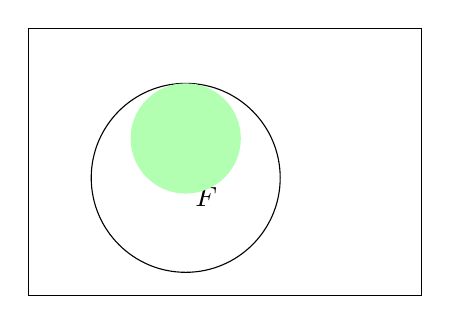
\begin{tikzpicture}[baseline]
        \draw (0,0) rectangle (5,3.4);
        \draw (2,1.5) circle (1.2cm) node[below right] {$F$};
        \fill[green!30] (2,2) circle (0.7cm) node[above] {$E$};
    \end{tikzpicture}
    &
    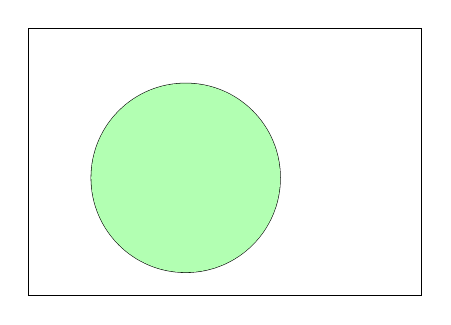
\begin{tikzpicture}[baseline]
        \draw (0,0) rectangle (5,3.4);
        \draw (2,1.5) circle (1.2cm) node[below right] {$F$};
        \fill[green!30] (2,1.5) circle (1.2cm) node[above] {$E$};
    \end{tikzpicture}
    &
    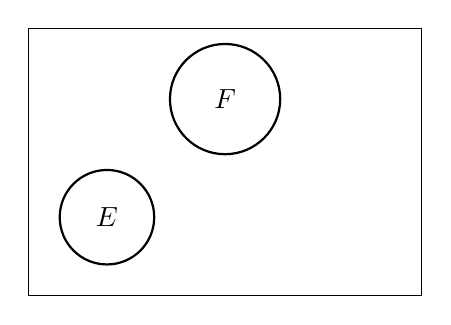
\begin{tikzpicture}[baseline]
        \draw (0,0) rectangle (5,3.4);
        \draw[thick] (1,1) circle (0.6cm) node {$E$};
        \draw[thick] (2.5,2.5) circle (0.7cm) node {$F$};
    \end{tikzpicture}
    \\
    
\end{tabular}
\end{center}

\section{What is Probability?}

There are three prominent ways to define probability.
In the three following subsections, these three definitions are explored.
Then an axiomatic definition of probability is given which is consistent with these three definitions.

\subsection{Classical Definition of Probability}\label{sec:classic}

In this definition, each elementary event of the sample space is considered to be equally likely to occur.
For example in rolling a fair die, all the events \( \{ 1 \}, \{ 2 \}, \{ 3 \}, \{ 4 \}, \{ 5 \} \) and \( \{ 6 \} \) have the same probability.
Or in tossing a coin (the random experiment in Example \autoref{exmp:coin_toss}), the elementary events \( \{ H \} \) and \( \{ T \} \) are all equally likely to happen,
which is consistent with our intuition of 50\% chance of occurring for each event.

This interpretation of probability goes back to Pierre-Simon Laplace, who wrote:
\begin{quote}
	The probability of an event is the ratio of the number of cases favorable to it, to the number of all cases possible when nothing leads us to expect that any one of these cases should occur more than any other, which renders them, for us, equally possible.
\FOOTNOTE{Laplace, Théorie analytique des probabilités, retrieved from \url{https://en.wikipedia.org/wiki/Classical_definition_of_probability}}
\end{quote}
So in this interpretation of probability, for an event \( E \subset S \), the probability of \( E \) is given by:
\begin{align*}
	P(E) = \frac{\text{number of outcomes in }E}{\text{total number of outcomes in }S}
\end{align*}

While we can assign a probability to each elementary event when the sample space consists of finitely many elements,
it is not possible when the elementary events are not equally likely to occur or the sample space is infinite like we saw in Example \autoref{exmp:heads_observe}.

\subsection{Frequentist Definition of Probability}

Consider a randon experiment in which we are interested in the occurrence of event \( E \).
Suppose this experiment is repeated \( n \) times under identical experimental conditions,
and event \( E \) occurs \( r \) times in total.
\( r \) and \( \frac{r}{n} \) are said to be the \keyterm{frequency} and \keyterm{relative frequency} of \( E \) in these
\( n \) trials, respectively.

As the number of trials \( n \) increases, the frequency \( r \) and consequently the relative frequency \( \frac{r}{n} \) changes as well.
However, empirical observations show that the relative frequency converges to a constant value, which in this interpretation is defined as the probability of \( E \).



The frequentist interpretation of probability may trace its earliest conceptual origins to Aristotle, who wrote
\begin{quote}
	the probable is that which for the most part happens
	\FOOTNOTE{Aristotle, Rhetoric, retrieved from \url{https://en.wikipedia.org/wiki/Frequentist_probability}}
\end{quote}
The frequentist interpretation of probability rose to dominance during the 19th century, becoming the foundation of classic statistical inference.

Let us reconsider the random experiment described in Example \autoref{exmp:three_balls_urn}.
According to the classical interpretation of probability, the probability of drawing a blue ball is \( \frac{1}{3} \).
However, if we don't know the urn's contents, we can determine the probability of drawing a red ball through a simple experiment.
By repeatedly drawing balls from the urn and calculating the relative frequency of drawing blue balls,
we observe that this ratio converges to \( \frac{1}{3} \) as the number of trials increases,
which is consistent with the classical definition of probabiltiy.
But the frequentist interpretation offers another advantage:
Suppose there are two blue balls, one green ball and one red ball in the urn.
Here, while the sample space remains \( \{ B, G, R \} \), the elementary events now have different probabilities
because there is an additional blue ball in the urn!
So while we cannot calculate the probability of drawing a blue ball using the classical definition,
we can determine it through the frequentist approach by performing many trials and observing the convergence of relative frequency.

While this interpretation sounds like a better approach to defining probability,
it faces several limitations. 
Consider, for instance, estimating the probability of precipitation occurring tomorrow.
There is, in fact, only one tomorrow;
we cannot conduct multiple trials of "tomorrow" to count rainy occurrences and determine their relative frequency.
Moreover, maintaining truly identical experimental conditions is practically impossible in most real-world scenarios.
Another fundamental challenge lies in determining how many trials are sufficient for the relative frequency to converge to a stable probability value.

\subsection{Epistemic Definition of Probability}

In this interpretation of probability, each observer assigns a subjective probability to an event based on their prior beliefs.
Reconsider the urn example from the previous subsection.
The experimenter draws a ball from the urn without revealing it to the observers.

An observer who saw the experimenter add an extra blue ball to the urn assigns a probability of \( \frac{2}{4} \) to the ball being blue.
Another observer, who previously knew the urn contained one blue, one green, and one red ball, assigns a probability of \( \frac{1}{3} \).
The experimenter, however, knows with certainty whether the ball is blue or not.

In the frequentist approach, the ball is either blue or not, and the probability is determined through repeated trials.
Thus, frequentists don't assign probabilities to single drawn balls.
In the epistemic perspective, however, each individual assigns a probability based on their existing knowledge.

\subsection{Axiomatic Definition of Probability}

Just like Euclidean geometry, where theorems are derived from a set of axioms taken as true\FOOTNOTE{\url{https://www.math.brown.edu/tbanchof/Beyond3d/chapter9/section01.html}},
modern probability theory is built upon axioms proposed by the Russian mathematician Andrey Kolmogorov in 1933.

A \keyterm{probability measure} on a sample space \( S \) is a function \( P(.) \) that assigns
to each event \( E \subset S \) a real number \( P(A) \), called the probability of \( A \),
satisfying the following three \keyterm{axioms of probability}:
\begin{itemize}
	\item for each event \( E \subset S \), the probability of \( A \) is non-negative, meaning \( P(E) \geq 0 \).
	\item the probability of \( S \) is 1, meaning \( P(S) = 1 \).
	\item if \( E_1, E_2, \ldots \) is a sequence of disjoint events, meaning \( E_i \cap E_j = \emptyset \) for each \( i \neq j \), then \( P(E_1 \cup E_2 \cup ...) = P(E_1) + P(E_2) + \ldots \).
\end{itemize}
The first axiom states that probabilities cannot be negative, which aligns with our intuition.
The second axiom indicates that since every experimental outcome belongs to the sample space, the event 
\( S \) must occur with probability 1.
The third axiom establishes that for any collection of disjoint events, the probability of their union equals the sum of their individual probabilities.

Different interpretations of probability remain consistent with the axiomatic definition.
Consider the frequentist approach:
\begin{itemize}
	\item Relative frequencies are non-negative, satisfying the first axiom.
	\item The relative frequency of \( S \) equals 1 in any number of trials, since every outcome belongs to the sample space.
	\item For mutually exclusive events, the relative frequency of their union equals the sum of their individual relative frequencies, as each outcome is counted only once.
\end{itemize}
Next, we prove some thorems using the axioms of probability.

\begin{theorem}\label{thm:imp_event}
	The probabiliy of impossible event, \( \emptyset \), is zero.
\end{theorem}
\begin{proof}
	Consider the sequence of events \( E_1, E_2, \ldots \) where \( E_1 = S \) and \( E_i = \emptyset \) for \( i > 1 \).
	Since the events in this sequence are mutually exclusive and \( S = \bigcup_{i = 1}^{\infty} E_i \), by the third axiom we have
	\[
	P(S) = P(\bigcup_{i = 1}^{\infty} A_i) = \sum_{i = 1}^{\infty} P(E_i) = P(S) + \sum_{i = 2}^{\infty} P(\emptyset) = P(S) + P(\bigcup_{i = 2}^{\infty}\emptyset) = P(S) + P(\emptyset)
	\]
	Cancelling \( P(S) \) from both sides we obtain \( P(\emptyset) = 0 \).
\end{proof}

\begin{theorem}\label{thm:finite_probs}
	For finitely many disjoint events \( E_1, E_2, \ldots, E_n \), we have
	\[
	P(\bigcup_{i = 1}^{n} E_i) = \sum_{i = 1}^{n} P(E_i)
	\]
\end{theorem}
\begin{proof}
	Consider the sequence of events \( E_1, E_2, \ldots \) where \( E_i = \emptyset \) for \( i > n \).
	Since all events in this sequence are mutually exclusive and \( \bigcup_{i = 1}^{n} E_i = \bigcup_{i = 1}^{\infty} E_i \),
	by applying the third axiom and \autoref{thm:imp_event} we have
	\begin{align*}
	P(\bigcup_{i = 1}^{n} E_i) = P(\bigcup_{i = 1}^{\infty} E_i) &= \sum_{i = 1}^{\infty} P(E_i)\\
	&= \sum_{i = 1}^{n} P(E_i) + \sum_{i = n + 1}^{\infty} P(E_i)\\
	&= \sum_{i = 1}^{n} P(E_i) + P(\bigcup_{i = n + 1}^{\infty} E_i)\\
	&= \sum_{i = 1}^{n} P(E_i) + P(\emptyset)\\
	&= \sum_{i = 1}^{n} P(E_i)
	\end{align*}
\end{proof}

\begin{theorem}
	For any event \( E \subset S \), \( P(E^\complement) = 1 - P(E) \).
\end{theorem}
\begin{proof}
	\( E \) and \( E^\complement \) are mutually exclusive and \( S = E \cup E^\complement \)
	since every element of the sample space is either in \( E \) or not.
	Thus, using the second axiom and \autoref{thm:finite_probs}, we have
	\begin{gather*}
		1 = P(S) = P(E \cup E^\complement) = P(E) + P(E^\complement)\\
		P(E^\complement) = 1 - P(E)
	\end{gather*}
\end{proof}
\begin{corollary}\label{cor:demorgan}
	Using De Morgan's laws in set theory, for any two events \( E, F \subset S \):
	\begin{align*}
		(E \cap F)^\complement = E^\complement \cup F^\complement\\
		(E \cup F)^\complement = E^\complement \cap F^\complement
	\end{align*}
	From these we can derive:
	\begin{align*}
		P(E^\complement \cup F^\complement) = P((E \cap F)^\complement) = 1 - P(E \cap F)\\
		P(E^\complement \cap F^\complement) = P((E \cup F)^\complement) = 1 - P(E \cup F)
	\end{align*}
\end{corollary}

\begin{theorem}\label{thm:difference_probs}
	For any two events \( F, E \subset S \), the equality \( P(F - E) = P(F) - P(E \cap F) \) holds.
\end{theorem}
\begin{proof}
	It can be shown that \( F = (F - E) \cup (E \cap F) \)
	where \( F - E \) and \( E \cap F \) are mutually exclusive.
	By \autoref{thm:finite_probs}:
	\begin{gather*}
		P(F) = P(F - E) + P(E \cap F)\\
		P(F - E) = P(F) - P(E \cap F)
	\end{gather*}
\end{proof}
\begin{corollary}\label{cor:subset_prob}
	If \( E \subset F \), then \( E \cap F = E \) and thus \( P(F - E) = P(F) - P(E) \).
\end{corollary}
\begin{corollary}
	If \( E \subset F \), the first axiom and Corollary \autoref{cor:subset_prob} yield \( P(E) \leq P(F) \).
	Replacing \( F \) with \( S \) and applying the second axiom gives \( P(E) \leq 1 \).
	Combined with the first axiom, this proves that for any event \( E \),
	\[
	0 \leq P(E) \leq 1
	\]
\end{corollary}

\begin{theorem}\label{thm:union_probs}
	For any two events \( E, F \subset S \), the equality \( P(E \cup F) = P(E) + P(F) - P(E \cap F) \) holds.
\end{theorem}
\begin{proof}
	It can be shown that \( E \cap F = E \cup (F - E) \)
	where \( E \) and \( F - E \) are mutually exclusive.
	By \autoref{thm:finite_probs} and \autoref{thm:difference_probs}:
	\[
		P(E \cup F) = P(E) + P(F - E) = P(E) + P(F) - P(E \cap F)
	\]
\end{proof}

\begin{exmp}
	Suppose \( E, F \) are two events from sample space \( S \) where \( P(E) = 0.6 \), \( P(F - E) = 0.3 \) and \( P(E \cap F) = 0.2 \).
	\begin{enumerate}
		\item What is \( P(F) \)?
		\item What is \( P(E \cup F) \)?
		\item What is \( P(E \cap F^\complement) \)?
		\item What is \( P(E \cap E^\complement) \)?
		\item What is \( P(E^\complement \cap F^\complement) \)?
	\end{enumerate}
\end{exmp}
\begin{solution}
	\begin{enumerate}
		\item From \autoref{thm:difference_probs}, we derive:
		\begin{align*}
			P(F) = P(F - E) + P(E \cap F) = 0.3 + 0.2 = 0.5
		\end{align*}
		\item By \autoref{thm:union_probs}:
		\begin{align*}
			P(E \cup F) = P(E) + P(F) - P(E \cap F) = 0.6 + 0.5 - 0.2 = 0.9
		\end{align*}
		\item From set theory, we have the equality \( E \cap F^\complement = E - F \).
		Intuitively, \( E \cap F^\complement \) and \( E - F \) both contain exactly those elements of \( S \) that belong to \( E \) but not to \( F \).
		Applying \autoref{thm:difference_probs} yields:
		\begin{align*}
			P(E \cap F^\complement) = P(E - F) = P(E) - P(F \cap E) = P(E) - P(E \cap F) = 0.6 - 0.2 = 0.4
		\end{align*}
		\item No element of \( S \) can simultaneously belong to \( E \) and not belong to it , thus \( E \cap E^\complement = \emptyset \).
		\autoref{thm:imp_event} implies:
		\begin{align*}
			P(E \cap E^\complement ) = P(\emptyset) = 0
		\end{align*}
		\item By Corollary \autoref{cor:demorgan}:
		\begin{align*}
			P(E^\complement \cap F^\complement) = 1 - P(E \cup F) = 1 - 0.9 = 0.1
		\end{align*}
	\end{enumerate}
\end{solution}

\begin{ex}
	Prove that for any two events \( E, F \subset S \), \( P(E^\complement \cup F) = 1 - P(E) + P(F \cap E) \).
\end{ex}

\section{Uniform Probability Model}

In a \keyterm{uniform probability model}, each elementary event has an equal probability.
So if the sample space has \( n(S) \) elements, then for each outcome \( e_i \in S \), we have:
\begin{align*}
	P(\{e_i\}) = \frac{1}{n(S)}
\end{align*}
If an event \( E \) contains \( n(E) \) elements,
we can express it as \( E = \bigcup_{j} \{e_j\} \), where each \( e_j \) is an element of \( S \) belonging to \( E \).
Applying \autoref{thm:finite_probs}:
\begin{align*}
	P(E) = P(\bigcup_{j} \{e_j\}) = \sum_{j} P(\{e_j\}) = \sum_{j} \frac{1}{n(S)} = \frac{n(E)}{n(S)}
\end{align*}
Comparing this with \autoref{sec:classic}, we observe that it is equivalent to Laplace's classical definition of probability.

\begin{exmp}
	In the coin toss random experiment from Example \autoref{exmp:coin_toss}, if the event of interest \( E \) is "observing heads",
	then \( P(E) = \frac{1}{2} \), since \( E = \{ H \} \) contains exactly one outcome out of two possible equally likely outcomes.
	Such a coin with equal probabilities of landing on heads or tails is called a \keyterm{fair coin}.
\end{exmp}

\begin{exmp}\label{exmp:three_fair_coins}
	In the random experiment of tossing three fair coins, the sample space is
	\( S = \{ HHH, HHT, HTH, HTT, THH, THT, TTH, TTT \} \).
	If the event of interest \( E \) is "observing at most two heads",
	then \( E = \{ HHT, HTH, HTT, THH, THT, TTH, TTT \} \) and consequently \( P(E) = \frac{7}{8} \).
\end{exmp}

\begin{exmp}
	In the die-throw random experiment from Example \autoref{exmp:fair_die}, if the event of interest \( E \) is "observing an odd number",
	then \( E = \{ 1, 3, 5 \} \) and thus \( P(E) = \frac{3}{6} = \frac{1}{2} \).
	A die with equally likely outcomes for all faces is called a \keyterm{fair die}.
\end{exmp}

\begin{exmp}\label{exmp:two_fair_dice}
	In the random experiment of tossing two fair six-sided dice, the sample space is
	\( S = \{ (1, 1), (1, 2), \ldots, (6, 5), (6, 6) \} \).
	If the event of interest \( E \) is "the sum of two dice equals 8",
	then \( E = \{ (2, 6), (3, 5), (4, 4), (5, 3), (6, 2) \} \) and consequently \( P(E) = \frac{5}{36} \).
\end{exmp}

\begin{ex}
	In Example \autoref{exmp:two_fair_dice}, what is the probability that the difference of two dice is 3?
\end{ex}

In the examples discussed above, we can easily count the elements in both the sample space and the event of interest.
However, consider modifying Example \autoref{exmp:three_fair_coins} where six fair coins are tossed instead of three,
or altering Example \autoref{exmp:two_fair_dice} to involve seven fair six-sided dice rather than two.
How many elements are in the sample space in these cases?
Attempting to list all possible combinations would quickly reveal what a tedious task this becomes.

The are some fundamental counting principles which aid us in these scenarios.
The \keyterm{multiplication principle} states that if a first task can be performed in \( m_1 \) ways,
and for each of these, a second task can be performed in \( m_2 \) ways independent from the previous task,
then the sequence of two tasks has \( m_1 \times m_2 \) possible outcomes.
This naturally extends to \( n \) sequential tasks,
where the total number of possible outcomes becomes \( m_1 \times m_2 \times \ldots \times m_n \).

\begin{exmp}
	A standard deck contains cards with four suits (\( \clubsuit, \vardiamondsuit, \spadesuit, \varheartsuit \)) and thirteen ranks (A, 1, 2, ..., 9, J, Q, K).
	How many total cards are in such a deck?
\end{exmp}
\begin{solution}
	We decompose the counting problem into two sequential tasks:
	selecting a suit and then selecting a rank.
	There are four ways to do the former and thirteen ways to do the latter, so in total there are \( 4 \times 13 = 52 \) such cards.
\end{solution}

The \keyterm{addition principle} states that if one task can be performed in \( n_1 \) ways and another distinct task in \( n_2 \) ways,
then either task can be done in \( n_1 + n_2 \) total ways.
For example, with three blue garments and seven green ones,
selecting either a blue or green garment can be done in \( 3 + 7 = 10 \) ways.
This result can be generalized to more than two tasks, analogous to the extension of the multiplication principle.

\begin{exmp}
	From a group of seven statisticians and five computer scientists, two people are randomly selected for a project.
	What is the probability that the team consists of one statistician and one computer scientist?
\end{exmp}
\begin{solution}
	The first person is chosen from 12 individuals, and the second from the remaining 11.
	So the sample space has \( n(S) = 12 \times 11 = 132 \) elements.
	The event \( E \) contains elements of \( S \) with one statistician and one computer scientist.
	So to count the number of elements in \( E \), we again decompose the problem into two tasks.
	First choosing one statistician and second choosing a conputer scientist,
	which can be done in \( 7 \times 5 = 35 \) ways.
	Or first choosing one computer scientist and then choosing a statistician,
	which can be done in \( 5 \times 7 = 35 \) ways.
	Since we have to choose a statistician first and then a computer scientist, or first a computer scientist and then a statistician,
	the addition principle implies \( n(E) = 35 + 35 = 70 \), yielding \( P(E) = \frac{70}{132} = \frac{35}{66} \).
\end{solution}

\section{Conditional Probability}

In previous sections, we examined basic probability examples.
But sometimes in our problems, we have some prior information.
In Example \autoref{exmp:two_fair_dice}, suppose we know beforehand that one die has come up 2.
Here, the event of interest becomes \( E \cap F \), where \( F \) is the event "one die comes up 2".
So we are interested in the probability of both \( E \) and \( F \) occurring, which is \( E \cap F = \{ (2, 6), (6, 2) \} \).
On the other hand, since we have information that one die has come up 2, the sample space is restricted from \( S \) to \( F \).
So the probability of \( E \) given we know \( F \) has occurred is \( \frac{n(E \cap F)}{n(F)} \).
By dividing the numerator and denominator by \( n(S) \), the desired probability becomes \( \frac{P(E \cap F)}{P(F)} \).
Since \( F = \{ (1, 2), (2, 1), (2, 2), (2, 3), (2, 4), (2, 5), (2, 6), (3, 2), (4, 2), (5, 2), (6, 2) \} \),
this probability is \( \frac{\frac{2}{36}}{\frac{11}{36}} = \frac{2}{11} \).

The \keyterm{conditional probability} of \( E \) given \( F \) is defined the same way in any probability model, not just the uniform one, and is denoted by \( P(E | F) = \frac{P(E \cap F)}{P(F)} \)
where \( P(F) > 0 \).
If \( P(F) = 0 \), \( P(E | F) \) would be undefined.

\begin{exmp}
	In Example \autoref{exmp:three_fair_coins}, let \( F \) be the event "observing exactly two tails".
	\begin{enumerate}
		\item What is \( P(E \cap F) \)?
		\item What is \( P(E | F) \)?
		\item What is \( P(F | E) \)?
	\end{enumerate}
\end{exmp}
\begin{solution}
	\begin{enumerate}
		\item First we note that \( F = \{ HTT, THT, TTH \} \).
		Thus, \( E \cap F = \{ HTT, THT, TTH \} \), yielding:
		\begin{align*}
			P(E \cap F) = \frac{n(E \cap F)}{n(S)} = \frac{3}{8}
		\end{align*}
		Here, we are interested in the event "observing at most two heads and exactly two tails" while the sample space is not restricted to a new one since we have no prior information.
		\item \begin{gather*}
			P(F) = \frac{n(F)}{n(S)} = \frac{3}{8}\\
			P(E | F) = \frac{P(E \cap F)}{P(F)} = \frac{\frac{3}{8}}{\frac{3}{8}} = 1
		\end{gather*}
		Unlike the previous part, we now have prior information that exactly two tails are observed. 
		By restricting our sample space to outcomes with exactly two tails, we are sure that zero or one head must be observed (and thus at most two heads total), which agrees with this result.
		\item \begin{gather*}
			P(F | E) = \frac{P(F \cap E)}{P(E)} = \frac{P(E \cap F)}{P(E)} = \frac{\frac{3}{8}}{\frac{7}{8}} = \frac{3}{7}
		\end{gather*}
		Let \( G \) be the event "observing at least one tail".
		Since \( G = E \), the two events are equal and so \( P(F | E) = P(F | G) \).
		In other words, \( P(F | E) \) is the same as the probability of observing exactly two tails given at least one tail is observed.
		The plausibility of observing exactly two tails after at least one tail is observed must increase,
		which is true since \( P(F | E) = \frac{3}{7} > \frac{3}{8} = P(F) \).
	\end{enumerate}
\end{solution}

Thus far, we have examined numerous examples of uniform probability models.
However, not all probability models are uniform.
Consider these cases:

\begin{exmp}
	Consider Example \autoref{exmp:three_balls_urn} with an urn containing three blue balls, five green balls, and two red balls.
	If we treat each ball as distinct, the sample space is \( S = \{ B_1, B_2, B_3, G_1, G_2, G_3, G_4, G_5, R_1, R_2 \} \).
	This forms a uniform probability model where \( P(\{B_1\}) = P(\{B_2\}) = \ldots = P(\{R_1\}) = P(\{R_2\}) = \frac{1}{10} \).
	However, if we are only interested in ball colors and not individual balls,
	the sample space reduces to \( S = \{ B, G, R \} \).
	Defining \( B = \{ B_1, B_2, B_3 \} \), \( G = \{ G_1, G_2, G_3, G_4, G_5 \} \) and \( R = \{ R_1, R_2 \} \),
	then \( P(B) = \frac{3}{10} \), \( P(G) = \frac{5}{10} = \frac{1}{2} \) and \( P(R) = \frac{2}{10} = \frac{1}{5} \),
	which is a non-uniform probability model.
\end{exmp}

\begin{exmp}\label{exmp:eye_color}
	The residents of a town have blue, green, brown, and amber eyes.
	When randomly selecting a resident, the event of interest is their eye color.
	The sample space for this experiment is \( S = \{ blue, green, brown, amber \} \).
	To determine the probabilities of elementary events, we conduct a survey by randomly sampling 500 people and recording their eye colors.
	The results are shown in the following table:
	\begin{center}
	\begin{tabular}{|l|r|r|r|r|r|}
	\hline
	\textbf{Eye Color} & \textbf{Blue} & \textbf{Green} & \textbf{Brown} & \textbf{Amber} & \textbf{Total} \\ 
	\hline
	Frequency & 125 & 65 & 290 & 20 & 500 \\
	Relative Frequency & 0.25 & 0.13 & 0.58 & 0.04 & 1.00 \\
	\hline
	\end{tabular}
	\end{center}
	{\footnotesize\textit{Note: Data reflects approximate global eye color distribution based on studies from the American Academy of Ophthalmology (2022)\FOOTNOTE{\url{https://www.aao.org/eye-health/tips-prevention/your-blue-eyes-arent-really-blue}}.}}
	
	Using the frequentist definition of probability and the survey data above, we obtain:
	\begin{align*}
		P(\{blue\}) = 0.25, P(\{green\}) = 0.13, P(\{brown\}) = 0.58, P(\{amber\}) = 0.04
	\end{align*}
	These unequal probabilities confirm this is not a uniform probability model.

	Using this model, we can answer questions like this:
	If there are 362500 residents in this town, how many are expected to have green eyes?
	
	Using the frequentist interpretation, we can answer this question through a simple calculation:
	\begin{align*}
		0.13 \times 362500 = 47125
	\end{align*}
\end{exmp}

The conditional probability and theorems derived from the three axioms of probability apply to any probability model.
The following example demonstrates this:

\begin{exmp}
	Suppose in Example \autoref{exmp:eye_color}, of people with blue eyes, 65 were female.
	One person is selected at random from the town.
	Given that the selected person has blue eyes, what is the probability that they are female?
\end{exmp}
\begin{solution}
	We define event \( E \) as "the selected pesron has blue eyes" and event \( F \) as "the selected person is female".
	Thus:
	\begin{gather*}
		P(F \cap E) = \frac{65}{500} = 0.13\\
		P(F | E) = \frac{P(F \cap E)}{P(E)} = \frac{0.13}{0.25} = 0.52
	\end{gather*}
\end{solution}

\section*{Glossary}

% Glossary Section 1

\chapter{Probability and Accuracy } 
\section{Probability}
\section{Conditional Probability \& Bayes’ Theorem}
\section{Prevalence, Relative Risk, Sensitivity, and Specificity}
\section*{Glossary}

\chapter{Descriptive Statistics } 
\section{Introduction to Data}
\section{Exploratory Data Analysis}
 \section*{Glossary} 


\chapter{Probability Distributions}
\section{Random Variables}
\section{ Binomial Distribution}
\section{Normal Distribution}
\section{Sampling Distribution and Central Limit Theorem}
\section*{Glossary} 


\chapter{Estimation}
\section{Point Estimation}
\section{Confidence Interval}
\section*{Glossary} 

\chapter{Estimation}
\section{Hypothesis Testing for One Sample}
\section{Hypothesis Testing for Two Variances}
\section{Hypothesis for Two Means}
\section{Hypothesis for Two Proportions}
\section*{Glossary} 

 \chapter{Hypothesis Testing}  \section*{Glossary} \begin{itemize}
	
	\item {\bf anecdotal evidence}: Evidence, often personal, that is collected
	casually rather than by a well-designed study.
	\index{anecdotal evidence}
	
	\item {\bf population}: A group we are interested in studying.
	``Population'' often refers to a
	group of people, but the term is used for other subjects,
	too.
	\index{population}
	
	\item {\bf cross-sectional study}: A study that collects data about a
	population at a particular point in time.
	\index{cross-sectional study}
	\index{study!cross-sectional}
	
	\item {\bf cycle}: In a repeated cross-sectional study, each repetition
	of the study is called a cycle.
	
	\item {\bf longitudinal study}: A study that follows a population over
	time, collecting data from the same group repeatedly.
	\index{longitudinal study}
	\index{study!longitudinal}
	
	\item {\bf record}: In a dataset, a collection of information about
	a single person or other subject.
	\index{record}
	
	\item {\bf respondent}: A person who responds to a survey.
	\index{respondent}
	
	\item {\bf sample}: The subset of a population used to collect data.
	\index{sample}
	
	\item {\bf representative}: A sample is representative if every member
	of the population has the same chance of being in the sample.
	\index{representative}
	
	\item {\bf oversampling}: The technique of increasing the representation
	of a sub-population in order to avoid errors due to small sample
	sizes.
	\index{oversampling}
	
	\item {\bf raw data}: Values collected and recorded with little or no
	checking, calculation or interpretation.
	\index{raw data}
	
	\item {\bf recode}: A value that is generated by calculation and other
	logic applied to raw data.
	\index{recode}
	
	\item {\bf data cleaning}: Processes that include validating data,
	identifying errors, translating between data types and
	representations, etc.
	
\end{itemize}

% Glossary Section 10


 \chapter{ }  \section*{Glossary} \begin{itemize}
	
	\item {\bf linear fit}: a line intended to model the relationship between
	variables.  \index{linear fit}
	
	\item {\bf least squares fit}: A model of a dataset that minimizes the
	sum of squares of the residuals.
	\index{least squares fit}
	
	\item {\bf residual}: The deviation of an actual value from a model.
	\index{residuals}
	
	\item {\bf goodness of fit}: A measure of how well a model fits data.
	\index{goodness of fit}
	
	\item {\bf coefficient of determination}: A statistic intended to
	quantify goodness of fit.
	\index{coefficient of determination}
	
	\item {\bf sampling weight}: A value associated with an observation in a
	sample that indicates what part of the population it represents.
	\index{sampling weight}
	
\end{itemize}

% Glossary Section 11


 \chapter{Probability and Accuracy}  \section*{Glossary} \begin{itemize}
	
	\item {\bf regression}: One of several related processes for estimating parameters
	that fit a model to data.
	\index{regression}
	
	\item {\bf dependent variables}: The variables in a regression model we would
	like to predict.  Also known as endogenous variables.
	\index{dependent variable}
	\index{endogenous variable}
	
	\item {\bf explanatory variables}: The variables used to predict or explain
	the dependent variables.  Also known as independent, or exogenous,
	variables.
	\index{explanatory variable}
	\index{exogenous variable}
	
	\item {\bf simple regression}: A regression with only one dependent and
	one explanatory variable.
	\index{simple regression}
	
	\item {\bf multiple regression}: A regression with multiple explanatory
	variables, but only one dependent variable.
	\index{multiple regression}
	
	\item {\bf linear regression}: A regression based on a linear model.
	\index{linear regression}
	
	\item {\bf ordinary least squares}: A linear regression that estimates
	parameters by minimizing the squared error of the residuals.
	\index{ordinary least squares}
	
	\item {\bf spurious relationship}: A relationship between two variables that is 
	caused by a statistical artifact or a factor, not included in the
	model, that is related to both variables.
	\index{spurious relationship}
	
	\item {\bf control variable}: A variable included in a regression to
	eliminate or ``control for'' a spurious relationship.
	\index{control variable}
	
	\item {\bf proxy variable}: A variable that contributes information to
	a regression model indirectly because of a relationship with another
	factor, so it acts as a proxy for that factor.
	\index{proxy variable}
	
	\item {\bf categorical variable}: A variable that can have one of a
	discrete set of unordered values.
	\index{categorical variable}
	
	\item {\bf join}: An operation that combines data from two DataFrames
	using a key to match up rows in the two frames.
	\index{join}
	\index{DataFrame}
	
	\item {\bf data mining}: An approach to finding relationships between
	variables by testing a large number of models.
	\index{data mining}
	
	\item {\bf logistic regression}: A form of regression used when the
	dependent variable is boolean.
	\index{logistic regression}
	
	\item {\bf Poisson regression}: A form of regression used when the
	dependent variable is a non-negative integer, usually a count.
	\index{Poisson regression}
	
	\item {\bf odds}: An alternative way of representing a probability, $p$, as
	the ratio of the probability and its complement, $p / (1-p)$.
	\index{odds}
	
\end{itemize}

% Glossary Section 12


 \chapter{ }  \section*{Glossary} \begin{itemize}
	
	\item {\bf time series}: A dataset where each value is associated with
	a timestamp, often a series of measurements and the times they
	were collected.
	\index{time series}
	
	\item {\bf window}: A sequence of consecutive values in a time series,
	often used to compute a moving average.
	\index{window}
	
	\item {\bf moving average}: One of several statistics intended to estimate
	the underlying trend in a time series by computing averages (of
	some kind) for a series of overlapping windows.
	\index{moving average}
	
	\item {\bf rolling mean}: A moving average based on the mean value in
	each window.
	\index{rolling mean}
	
	\item {\bf exponentially-weighted moving average (EWMA)}: A moving
	average based on a weighted mean that gives the highest weight
	to the most recent values, and exponentially decreasing weights
	to earlier values. \index{exponentially-weighted moving average} \index{EWMA}
	
	\item {\bf span}: A parameter of EWMA that determines how quickly the
	weights decrease.
	\index{span}
	
	\item {\bf serial correlation}: Correlation between a time series and
	a shifted or lagged version of itself.
	\index{serial correlation}
	
	\item {\bf lag}: The size of the shift in a serial correlation or
	autocorrelation.
	\index{lag}
	
	\item {\bf autocorrelation}: A more general term for a serial correlation
	with any amount of lag.
	\index{autocorrelation function}
	
	\item {\bf autocorrelation function}: A function that maps from lag to
	serial correlation.
	
	\item {\bf stationary}: A model is stationary if the parameters and the
	distribution of residuals does not change over time.
	\index{model}
	\index{stationary model}
	
\end{itemize}

% Glossary Section 13


 \chapter{ }  \section*{Glossary} \begin{itemize}
	
	\item {\bf survival analysis}: A set of methods for describing and
	predicting lifetimes, or more generally time until an event occurs.
	\index{survival analysis}
	
	\item {\bf survival curve}: A function that maps from a time, $t$, to the
	probability of surviving past $t$.
	\index{survival curve}
	
	\item {\bf hazard function}: A function that maps from $t$ to the fraction
	of people alive until $t$ who die at $t$.
	\index{hazard function}
	
	\item {\bf Kaplan-Meier estimation}: An algorithm for estimating hazard and
	survival functions.
	\index{Kaplan-Meier estimation}
	
	\item {\bf cohort}: a group of subjects defined by an event, like date of
	birth, in a particular interval of time.
	\index{cohort}
	
	\item {\bf cohort effect}: a difference between cohorts.
	\index{cohort effect}
	
	\item {\bf NBUE}: A property of expected remaining lifetime, ``New
	better than used in expectation.''
	\index{NBUE}
	
	\item {\bf UBNE}: A property of expected remaining lifetime, ``Used
	better than new in expectation.''
	\index{UBNE}
	
\end{itemize}

% Glossary Section 2


 \chapter{ }  \section*{Glossary} \begin{itemize}
	
	\item {\bf distribution}: The values that appear in a sample
	and the frequency of each.
	\index{distribution}
	
	\item {\bf histogram}: A mapping from values to frequencies, or a graph
	that shows this mapping.
	\index{histogram}
	
	\item {\bf frequency}: The number of times a value appears in a sample.
	\index{frequency}
	
	\item {\bf mode}: The most frequent value in a sample, or one of the
	most frequent values.
	\index{mode}
	
	\item {\bf normal distribution}: An idealization of a bell-shaped distribution;
	also known as a Gaussian distribution. 
	\index{Gaussian distribution}
	\index{normal distribution}
	
	\item {\bf uniform distribution}: A distribution in which all values have
	the same frequency.
	\index{uniform distribution}
	
	\item {\bf tail}: The part of a distribution at the high and low extremes.
	\index{tail}
	
	\item {\bf central tendency}: A characteristic of a sample or population;
	intuitively, it is an average or typical value. 
	\index{central tendency}
	
	\item {\bf outlier}: A value far from the central tendency.
	\index{outlier}
	
	\item {\bf spread}: A measure of how spread out the values in a distribution
	are.
	\index{spread}
	
	\item {\bf summary statistic}: A statistic that quantifies some aspect
	of a distribution, like central tendency or spread.
	\index{summary statistic}
	
	\item {\bf variance}: A summary statistic often used to quantify spread.
	\index{variance}
	
	\item {\bf standard deviation}: The square root of variance, also used
	as a measure of spread.
	\index{standard deviation}
	
	\item {\bf effect size}: A summary statistic intended to quantify the size
	of an effect like a difference between groups.
	\index{effect size}
	
	\item {\bf clinically significant}: A result, like a difference between groups,
	that is relevant in practice.
	\index{clinically significant}
	
\end{itemize}

% Glossary Section 3


 \chapter{ }  \section*{Glossary} \begin{itemize}
	
	\item {\bf Probability mass function (PMF)}: a representation of a distribution
	as a function that maps from values to probabilities.
	\index{PMF}
	\index{probability mass function}
	
	\item {\bf probability}: A frequency expressed as a fraction of the sample
	size.
	\index{frequency}
	\index{probability}
	
	\item {\bf normalization}: The process of dividing a frequency by a sample
	size to get a probability.
	\index{normalization}
	
	\item {\bf index}: In a pandas DataFrame, the index is a special column
	that contains the row labels.
	\index{pandas}
	\index{DataFrame}
	
\end{itemize}

% Glossary Section 4


 \chapter{ }  \section*{Glossary} \begin{itemize}
	
	\item {\bf percentile rank}: The percentage of values in a distribution that are
	less than or equal to a given value.
	\index{percentile rank}
	
	\item {\bf percentile}: The value associated with a given percentile rank.
	\index{percentile}
	
	\item {\bf cumulative distribution function (CDF)}: A function that maps
	from values to their cumulative probabilities.  $CDF(x)$ is the
	fraction of the sample less than or equal to $x$.  \index{CDF}
	\index{cumulative probability}
	
	\item {\bf inverse CDF}: A function that maps from a cumulative probability,
	$p$, to the corresponding value.
	\index{inverse CDF}
	\index{CDF, inverse}
	
	\item {\bf median}: The 50th percentile, often used as a measure of central
	tendency.  \index{median}
	
	\item {\bf interquartile range}: The difference between
	the 75th and 25th percentiles, used as a measure of spread.
	\index{interquartile range}
	
	\item {\bf quantile}: A sequence of values that correspond to equally spaced
	percentile ranks; for example, the quartiles of a distribution are
	the 25th, 50th and 75th percentiles.
	\index{quantile}
	
	\item {\bf replacement}: A property of a sampling process. ``With replacement''
	means that the same value can be chosen more than once; ``without
	replacement'' means that once a value is chosen, it is removed from
	the population.
	\index{replacement}
	
\end{itemize}

% Glossary Section 5


 \chapter{ }  \section*{Glossary} \begin{itemize}
	
	\item {\bf empirical distribution}: The distribution of values in a sample.
	\index{empirical distribution} \index{distribution!empirical}
	
	\item {\bf analytic distribution}: A distribution whose CDF is an analytic
	function.
	\index{analytic distribution}
	\index{distribution!analytic}
	
	\item {\bf model}: A useful simplification.  Analytic distributions are
	often good models of more complex empirical distributions.
	\index{model}
	
	\item {\bf interarrival time}: The elapsed time between two events.
	\index{interarrival time}
	
	\item {\bf complementary CDF}: A function that maps from a value, $x$,
	to the fraction of values that exceed $x$, which is $1 - CDF(x)$.
	\index{complementary CDF} \index{CDF!complementary} \index{CCDF}
	
	\item {\bf standard normal distribution}: The normal distribution with
	mean 0 and standard deviation 1.
	\index{standard normal distribution}
	
	\item {\bf normal probability plot}: A plot of the values in a sample versus
	random values from a standard normal distribution.
	\index{normal probability plot}
	\index{plot!normal probability}
	
\end{itemize}

% Glossary Section 6


 \chapter{ }  \section*{Glossary} \begin{itemize}
	
	\item {\bf Probability density function (PDF)}: The derivative of a continuous CDF,
	a function that maps a value to its probability density.
	\index{PDF}
	\index{probability density function}
	
	\item {\bf Probability density}: A quantity that can be integrated over a
	range of values to yield a probability.  If the values are in units
	of cm, for example, probability density is in units of probability
	per cm.
	\index{probability density}
	
	\item {\bf Kernel density estimation (KDE)}: An algorithm that estimates a PDF
	based on a sample.
	\index{kernel density estimation}
	\index{KDE}
	
	\item {\bf discretize}: To approximate a continuous function or distribution
	with a discrete function.  The opposite of smoothing.
	\index{discretize}
	
	\item {\bf raw moment}: A statistic based on the sum of data raised to a power.
	\index{raw moment}
	
	\item {\bf central moment}: A statistic based on deviation from the mean,
	raised to a power.
	\index{central moment}
	
	\item {\bf standardized moment}: A ratio of moments that has no units.
	\index{standardized moment}
	
	\item {\bf skewness}: A measure of how asymmetric a distribution is.
	\index{skewness}
	
	\item {\bf sample skewness}: A moment-based statistic intended to quantify
	the skewness of a distribution.
	\index{sample skewness}
	
	\item {\bf Pearson's median skewness coefficient}: A statistic intended to
	quantify the skewness of a distribution based on the median, mean,
	and standard deviation.
	\index{Pearson median skewness}
	
	\item {\bf robust}: A statistic is robust if it is relatively immune to the
	effect of outliers.
	\index{robust}
	
\end{itemize}

% Glossary Section 7


 \chapter{Probability and Accuracy } \section{Probability}
 \section{Conditional Probability \& Bayes’ Theorem}
 \section{Prevalence, Relative Risk, Sensitivity, and Specificity}
  \section*{Glossary} \begin{itemize}
	
	\item {\bf scatter plot}: A visualization of the relationship between
	two variables, showing one point for each row of data.
	\index{scatter plot}
	
	\item {\bf jitter}: Random noise added to data for purposes of
	visualization.
	\index{jitter}
	
	\item {\bf saturation}: Loss of information when multiple points are
	plotted on top of each other. 
	\index{saturation}
	
	\item {\bf correlation}: A statistic that measures the strength of the
	relationship between two variables.
	\index{correlation}
	
	\item {\bf standardize}: To transform a set of values so that their mean is 0 and
	their variance is 1.
	\index{standardize}
	
	\item {\bf standard score}: A value that has been standardized so that it is
	expressed in standard deviations from the mean.
	\index{standard score}
	\index{standard deviation}
	
	\item {\bf covariance}: A measure of the tendency of two variables
	to vary together.
	\index{covariance}
	
	\item {\bf rank}: The index where an element appears in a sorted list.
	\index{rank}
	
	\item {\bf randomized controlled trial}: An experimental design in which subjects
	are divided into groups at random, and different groups are given different
	treatments.
	\index{randomized controlled trial}
	
	\item {\bf treatment group}: A group in a controlled trial that receives
	some kind of intervention.
	\index{treatment group}
	
	\item {\bf control group}: A group in a controlled trial that receives no
	treatment, or a treatment whose effect is known.
	\index{control group}
	
	\item {\bf natural experiment}: An experimental design that takes advantage of
	a natural division of subjects into groups in ways that are at least
	approximately random.
	\index{natural experiment}
	
\end{itemize}

% Glossary Section 8


 \chapter{Descriptive Statistics } \section{Introduction to Data}
 \section{Exploratory Data Analysis} \section*{Glossary} \begin{itemize}
	
	\item {\bf estimation}: The process of inferring the parameters of a distribution
	from a sample.
	\index{estimation}
	
	\item {\bf estimator}: A statistic used to estimate a parameter.
	\index{estimation}
	
	\item {\bf mean squared error (MSE)}: A measure of estimation error.
	\index{mean squared error}
	\index{MSE}
	
	\item {\bf root mean squared error (RMSE)}: The square root of MSE,
	a more meaningful representation of typical error magnitude.
	\index{mean squared error}
	\index{MSE}
	
	\item {\bf maximum likelihood estimator (MLE)}: An estimator that computes the
	point estimate most likely to be correct.
	\index{MLE}
	\index{maximum likelihood estimator}
	
	\item {\bf bias (of an estimator)}: The tendency of an estimator to be above or
	below the actual value of the parameter, when averaged over repeated
	experiments.  \index{biased estimator}
	
	\item {\bf sampling error}: Error in an estimate due to the limited
	size of the sample and variation due to chance. \index{point estimation}
	
	\item {\bf sampling bias}: Error in an estimate due to a sampling process
	that is not representative of the population. \index{sampling bias}
	
	\item {\bf measurement error}: Error in an estimate due to inaccuracy collecting
	or recording data. \index{measurement error}
	
	\item {\bf sampling distribution}: The distribution of a statistic if an
	experiment is repeated many times.  \index{sampling distribution}
	
	\item {\bf standard error}: The RMSE of an estimate,
	which quantifies variability due to sampling error (but not
	other sources of error).
	\index{standard error}
	
	\item {\bf confidence interval}: An interval that represents the expected
	range of an estimator if an experiment is repeated many times.
	\index{confidence interval} \index{interval!confidence}
	
\end{itemize}

% Glossary Section 9


 \chapter{Probability Distributions}
  \section{Random Variables}
  \section{ Binomial Distribution}
 \section{Normal Distribution}
 \section{Sampling Distribution and Central Limit Theorem}
  \section*{Glossary} \begin{itemize}
	
	\item {\bf hypothesis testing}: The process of determining whether an apparent
	effect is statistically significant.
	\index{hypothesis testing}
	
	\item {\bf test statistic}: A statistic used to quantify an effect size.
	\index{test statistic}
	\index{effect size}
	
	\item {\bf null hypothesis}: A model of a system based on the assumption that
	an apparent effect is due to chance.
	\index{null hypothesis}
	
	\item {\bf p-value}: The probability that an effect could occur by chance.
	\index{p-value}
	
	\item {\bf statistically significant}: An effect is statistically
	significant if it is unlikely to occur by chance.
	\index{significant} \index{statistically significant}
	
	\item {\bf permutation test}: A way to compute p-values by generating
	permutations of an observed dataset.
	\index{permutation test}
	
	\item {\bf resampling test}: A way to compute p-values by generating
	samples, with replacement, from an observed dataset.
	\index{resampling test}
	
	\item {\bf two-sided test}: A test that asks, ``What is the chance of an effect
	as big as the observed effect, positive or negative?''
	
	\item {\bf one-sided test}: A test that asks, ``What is the chance of an effect
	as big as the observed effect, and with the same sign?''
	\index{one-sided test}
	\index{two-sided test}
	\index{test!one-sided}
	\index{test!two-sided}
	
	\item {\bf chi-squared test}: A test that uses the chi-squared statistic as
	the test statistic.
	\index{chi-squared test}
	
	\item {\bf false positive}: The conclusion that an effect is real when it is not.
	\index{false positive}
	
	\item {\bf false negative}: The conclusion that an effect is due to chance when it
	is not.
	\index{false negative}
	
	\item {\bf power}: The probability of a positive test if the null hypothesis
	is false.
	\index{power}
	\index{null hypothesis}
	
\end{itemize}


%%%%%%%%%%%%%%  references %%%%%%%%%%%%%%

%\chapter{References}
%\printbibliography[heading=none]
%\printindex
\afterpage{\blankpage}

%back cover
%\includepdf[noautoscale=false,pages=-]{../img/backCover.pdf}
%\pagenumbering{gobble} 




\end{document}